
\section{Analyse von Filterschaltungen mit SFDs}

Aktive Filterschaltungen (mit OpAmps) können mittels Signalflussdiagrammen (SFDs) analysiert werden. Dazu wird die gesamte Schaltung
in einzelne Komponenten aufgeteilt. Diese Komponenten werden dann mit Impedanz- bzw. Admittanzfunktionen abgebildet.
Um die Übertragungsfunktion (UTF) der gesamten Schaltung zu erhalten, muss die \textbf{Regel von Mason} angewendet werden.

\subsection{Eingangsadmittanzen / (Eingangsimpedanzen)}

\textbf{Hinweis:} Es wird normalerweise mit Eingangs\textbf{admittanzen} gearbeitet!

\begin{ctabular}{lll}
    \textbf{Komponente} & \textbf{Admittanz} $\bm{Y}$       & (\textbf{Impedanz} $\bm{Z}$) \\
    \midrule
    Widerstand $R$      & $Y_{\rm res} = \frac{1}{R}$           & ($Z_{\rm res} = R$  )\\
    Kapazität $C$       & $Y_{\rm cap} = s \cdot C$             & ($Z_{\rm cap} = \frac{1}{s \cdot C}$)\\
    Induktivität $L$    & $Y_{\rm ind} = \frac{1}{s \cdot L}$   & ($Z_{\rm ind} = s \cdot L$)
\end{ctabular}


\subsection{OpAmp Impedanzfunktionen}

\textbf{Hinweis:} Es geht um \textbf{negatives Feedback} bzw. \textbf{Gegenkopplung}

\begin{ctabular}{ll}
    \textbf{Schaltung (Feedback)}       & \textbf{Impedanz} $\bm{Z}$ \\
    \midrule
    Widerstand $R_f$ im Feedback        & $Z_{\rm op} = - R_f$ \\
    Kapazität $C_f$ im Feedback         & $Z_{\rm op} = - \frac{1}{s \cdot C_f}$ \\
    $R_f C_f$ (parallel) im Feedback    & $Z_{\rm op} = - \frac{R_f}{1 + s \cdot C_f \cdot R_f}$
\end{ctabular}


\example{Summierender Verstärker}

\begin{minipage}[c]{0.4\columnwidth}
    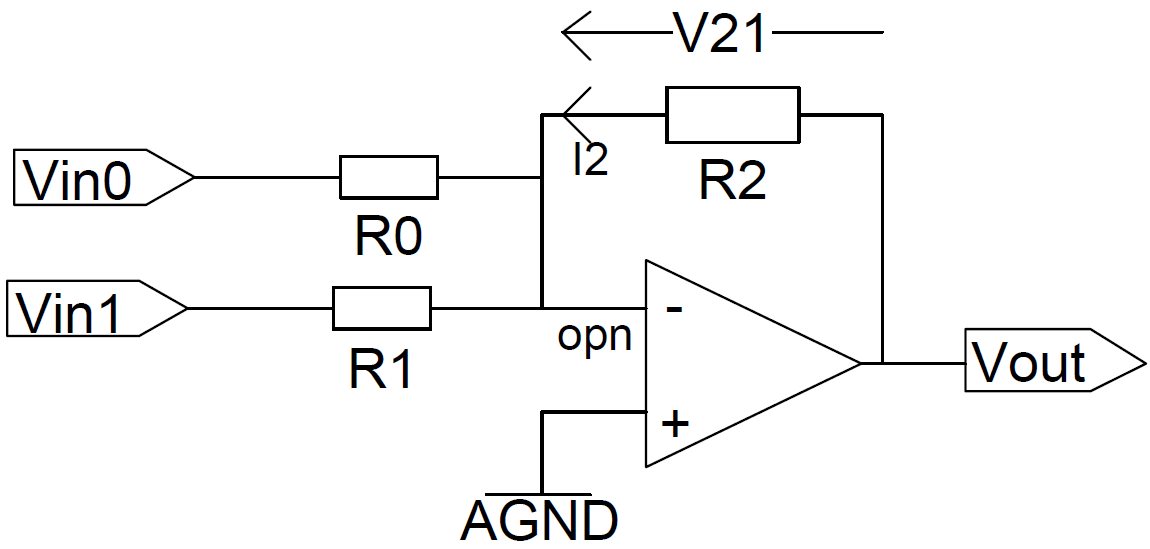
\includegraphics[width=\columnwidth]{images/summierender_verstaerker.png}
\end{minipage}
\hfill
\begin{minipage}[c]{0.58\columnwidth}
    \begin{center}
        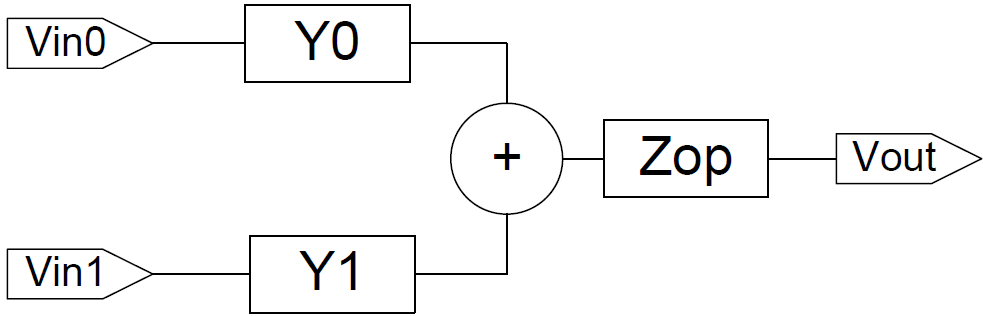
\includegraphics[width=0.8\columnwidth]{images/summierender_verstaerker_sfd.png}
    \end{center}
    $$ V_{\rm out} = Z_{\rm op} \cdot (Y_0 \cdot V_{\rm in0} + Y_1 \cdot V_{\rm in1}) $$
\end{minipage}

$$ Y_0 = \frac{1}{R_0} \qquad Y_1 = \frac{1}{R_1} \qquad Z_{\rm op} = - R_f $$


\example{Aktiver Tiefpass 1. Ordnung}

\begin{minipage}[c]{0.4\columnwidth}
    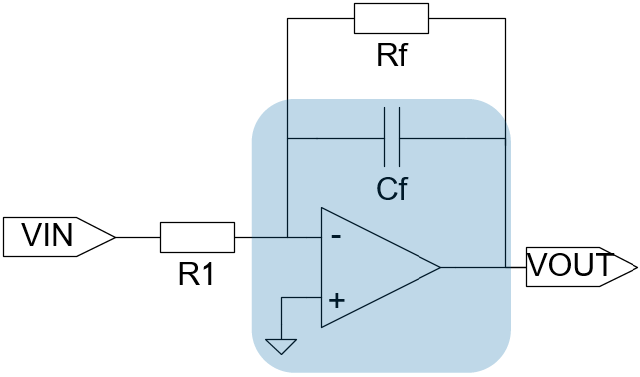
\includegraphics[width=\columnwidth]{images/filter_signalflussdiagramme_tiefpass_ordnung_1.png}
\end{minipage}
\hfill
\begin{minipage}[c]{0.48\columnwidth}
    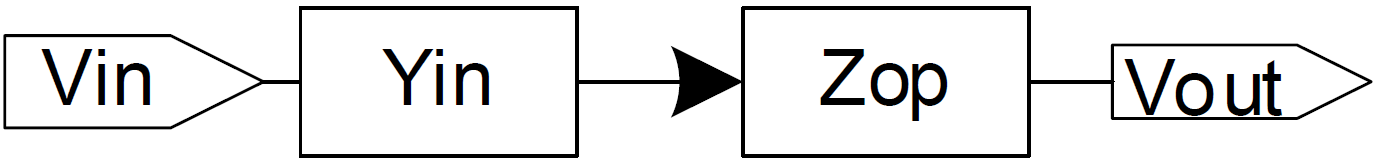
\includegraphics[width=\columnwidth]{images/filter_signalflussdiagramme_tiefpass_ordnung_1_sfd.png}
    $$ Y_{\rm in} = \frac{1}{R_1} \qquad Z_{\rm op} = - \frac{R_f}{1 + s \cdot C_f \cdot R_f} $$
\end{minipage}

$$ G(s)= \frac{V_{\rm out}}{V_{\rm in}} = Y_{\rm in} \cdot Z_{\rm op} =- \frac{R_f}{1 + s \cdot C_f \cdot R_f} \cdot \frac{1}{R_1} $$


\subsection{Regel von Mason (vereinfacht)}

$$ \boxed{ \text{UTF:} \quad G(s) = \frac{V_{\rm out}}{V_{\rm in}} = \frac{\text{Produkt der Transmittanzen im Vorwärtspfad}}{1 - \text{Summe aller Schleifentransmittanzen}} }$$


\example{Analyse Bandpass mittels SFD und Regel von Mason}

\begin{minipage}[c]{0.48\columnwidth}
    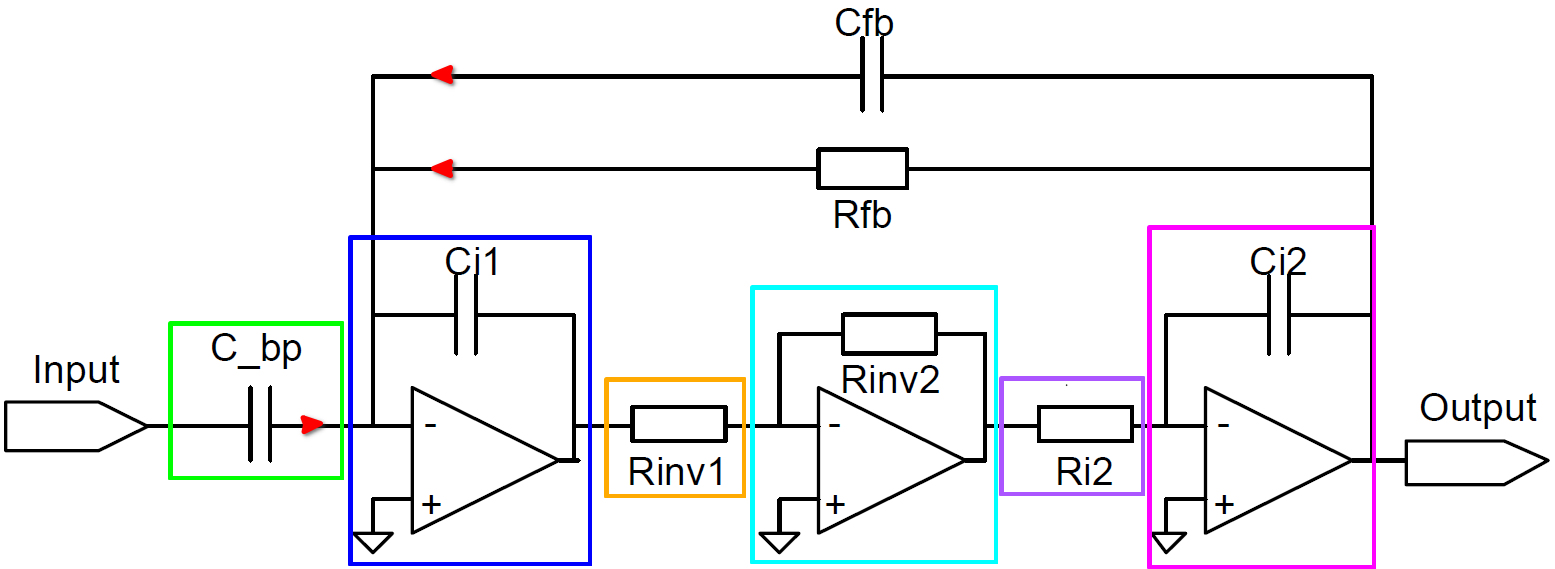
\includegraphics[width=\columnwidth]{images/signalflussdiagramme_bandpass_schaltung.png}
\end{minipage}
\hfill
\begin{minipage}[c]{0.48\columnwidth}
    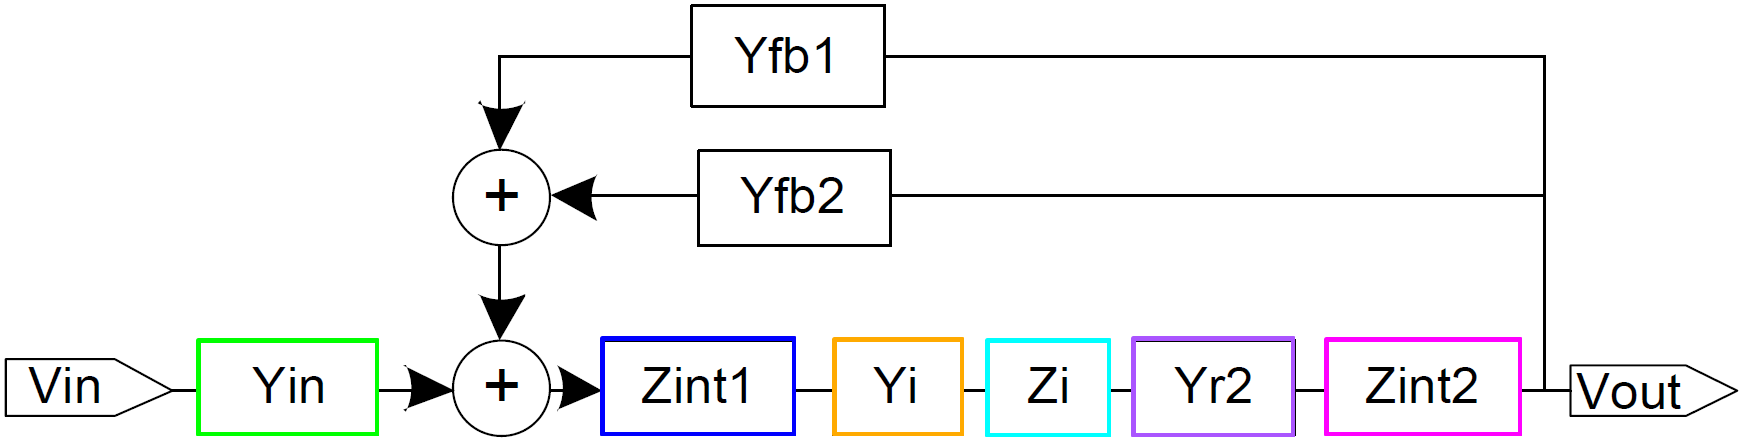
\includegraphics[width=\columnwidth]{images/signalflussdiagramme_bandpass_blockschaltbild.png}
\end{minipage}

$$ G(s) = \frac{V_{\rm out}}{V_{\rm in}} = \frac{Y_{\rm in} \cdot Z_{\rm int1} \cdot Y_i \cdot Z_i \cdot Y_{r2} \cdot Z_{\rm int2} }
    {1 - (Y_{\rm fb1} - Y_{\rm fb2}) \cdot Z_{\rm int1} \cdot Y_i \cdot Z_i \cdot Y_{r2} \cdot Z_{\rm int2} } $$
